\documentclass{beamer}
%\documentclass[draft]{beamer} %Zum schnelleren Kompilieren beim Entwickeln
%\documentclass[notes=show]{beamer}
\usepackage[utf8]{inputenc}
\usepackage{ngerman}
\usepackage{rotating}
\usepackage{verbatim}
\usepackage{latexsym}
\usepackage{color}
\usepackage{graphicx}
\usepackage{tabularx}
\usepackage{ragged2e}
\usepackage{eurosym}
\definecolor{boxgray}{gray}{0.88}
\selectlanguage{german}

\usepackage{listings}
\definecolor{listinggray}{gray}{0.94}
\lstset{backgroundcolor=\color{listinggray}}

\usetheme{Frankfurt}



% LaTeX-interne Einstellungen zum Umbruch etc.
% \nofiles    % Inhaltsverzeichnis nicht ändern.
\hbadness 10000
\sloppy
\frenchspacing

\usecolortheme{default}
% das ist die leiste mit dem frametitel
\setbeamercolor{palette primary}{use=structure,fg=white,bg=orange}
%Das ist die leiste ganz oben
\setbeamercolor{palette quaternary}{fg=orange,bg=black}

\newcolumntype{Y}{>{\centering\arraybackslash}X}%
\newcolumntype{Z}{>{\hfill\arraybackslash}X}%

\usepackage{amsmath,amssymb}

\setbeamercovered{dynamic}

%notes:
\setbeamertemplate{note page}[plain] 
%compressed


% Metadaten von Vortrag
\newcommand{\datum}{2012-07-19}
\newcommand{\autor}{Michael Stapelberg, Felix Bruckner, Pascal Krause}
\newcommand{\vorlesung}{Parallele Rechnerarchitekturen}
\newcommand{\semester}{SS2012}
\newcommand{\ort}{Hochschule Mannheim}

\title[]{SRA/ALR Prüfung\\ \ort}
\author{\autor}
\institute{Fakultät für Informatik\\
           Hochschule Mannheim\\}
\date{\datum}
\beamertemplatetransparentcovereddynamic
\setbeamerfont{note page}{size=\small}
%\renewcommand{\>}{\rangle}
%\newcommand{\<}{\langle} 
%\usebeamercolor[fg]{[page number]}

\setbeamertemplate{navigation symbols}{}
%\setbeamertemplate{note page}{}

%Zum Abschalten der kleinen Navigationsleiste am unteren Rand reicht folgende Zeile aus:
%\beamertemplatenavigationsymbolsempty

\setbeamersize{text margin left=0.2cm}
\setbeamersize{text margin right=0.25cm}
\setbeamersize{sidebar width right=0cm}
\setbeamersize{sidebar width left=0cm}

%Inhalt der Fußzeile festlegen
\setbeamertemplate{footline}
{
\setbeamercolor{bgcolor}{fg=black,bg=white}
\begin{beamercolorbox}{bgcolor}
\hspace*{0.2cm}
% \copyright 
\autor\ -- \vorlesung\ -- \ort\ -- \semester
\hfill
%  \insertslidenavigationsymbol
%  \insertframenavigationsymbol
%  \insertsubsectionnavigationsymbol
%  \insertsectionnavigationsymbol
%  \insertdocnavigationsymbol
%  \insertbackfindforwardnavigationsymbol
 \hfill\insertframenumber/\inserttotalframenumber
 \hspace*{0.2cm}
\end{beamercolorbox}

}

%\newcommand{\markNote}[1]{	\textsuperscript{\tiny [#1]} }
\newcommand{\markNote}[1]{	 }

% Bei jeder Section ein Inhaltsverzeichnis ausgeben
 \AtBeginSection[]{
 \begin{frame}
 %\frametitle{Outline}
 \tableofcontents[current] % Nur die sections ausgeben
 \end{frame}
 }

% Die Zeile definieren, die ganz oben ist und die Abschnitte enthält
% Das sind die Maße wenn es die Folie "nächste Vorlesung gibt"
% \setbeamertemplate{headline}
% {%
%   \begin{beamercolorbox}{section in head/foot}
%     \vskip5pt\insertnavigation{12.4cm}\vskip5pt
%   \end{beamercolorbox}%
% }

%\setbeamertemplate{headline}
%{%
%  \begin{beamercolorbox}{section in head/foot}
%    \vskip5pt\insertnavigation{12.75cm}\vskip5pt
%  \end{beamercolorbox}%
%}

\begin{document}

% Deckblatt generieren
\begin{frame}
\titlepage
\end{frame}

% Inhaltsverzeichnis am Anfang des Dokuments
\begin{frame}
  %\frametitle{Heute}
  %\tableofcontents[hideallsubsections]  % Nur die sections ausgeben
  \tableofcontents                       % sections und subsections ausgeben
\end{frame}

%Allgemeines zu S3
\section{Allgemeines}
\subsection{Unser Projekt}
\begin{frame}
\frametitle{Projektidee: Objekttracing}

\hspace*{0,3cm}{Jede einigermaßen ebene Fläche soll als Whiteboard dienen können.}

\vspace*{0,8cm}

\begin{itemize}
	\item Schwierigkeiten
	\begin{itemize}
		\item Qualität des Tiefenbildes zu schlecht
		\item Pure Farberkennung zu viele false-positives
	\end{itemize}
	\item Lösungsansatz
		\begin{itemize}
		\item Aufbereitung der Daten durch Anwenden von Filtern
	\end{itemize}
\end{itemize}
\end{frame}

\subsection{Architektur}

\begin{frame}
\frametitle{Architektur}
\hspace*{0.9cm}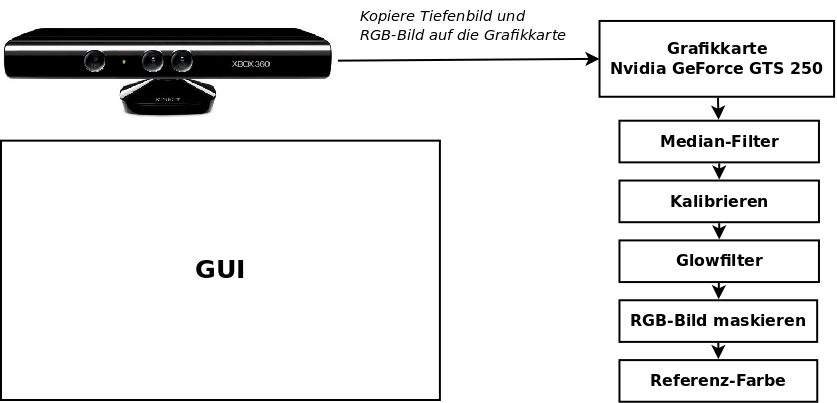
\includegraphics[width=10.5cm]{architektur.png}

\end{frame}

\subsection{Vorgehen}

\begin{frame}
\frametitle{Vorgehen}

\begin{itemize}
	\item Suchen eines open-source SDKs
	\item Erforschen der Kinect
	\item Suchen nach Problemlösungen
	\item Validieren der Lösungen (CPU)
	\item Portieren der Lösungen auf GPU
	\begin{itemize}
		\item Programmaufbau an CUDA anpassen 
		\item Algorithmen für CUDA optimieren
	\end{itemize}
	
\end{itemize}
\end{frame}

\section{Hardware}

\subsection{Kinect}
\begin{frame}
\frametitle{Kinect}

\hspace*{1.8cm}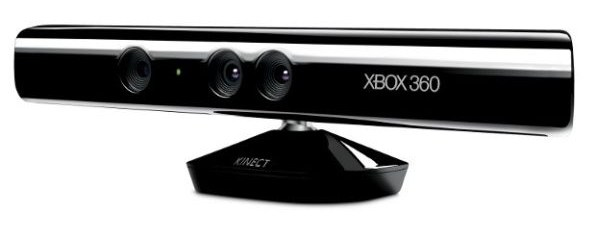
\includegraphics[width=8.5cm]{kin.jpg}

\begin{itemize}
	\item Sensoren
	\begin{itemize}
		\item 640x480 \@ 30Hz Farbbild (RGB)
		\item 640x480 \@ 30Hz Tiefenbild
	\end{itemize}
	\item Genauigkeit
	\begin{itemize}
		\item Genauigkeit ab 50cm ca. 1,5mm
		\item Genauigkeit ab 5m ca. 5cm
	\end{itemize}
\end{itemize}
\end{frame}

\subsection{Grafikkarte}
\begin{frame}
\frametitle{Grafikkarte}

\hspace*{1.8cm}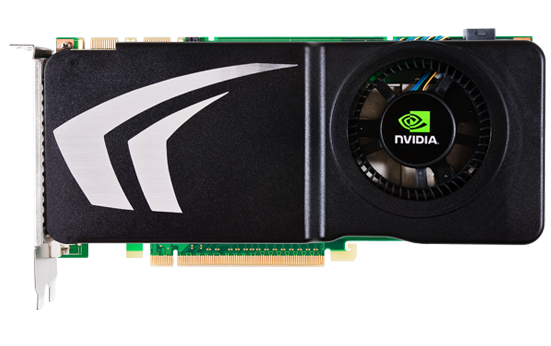
\includegraphics[width=8.5cm]{gts250.png}

\begin{itemize}
	\item Nvidia GeForce GTS 250
	\item 16 Multiprozessoren mit je 8 Cores
	\item 1024 MB Device-Memory	
\end{itemize}
\end{frame}

\subsection{Handschuh}
\begin{frame}
\frametitle{Handschuh}

\hspace*{2.5cm}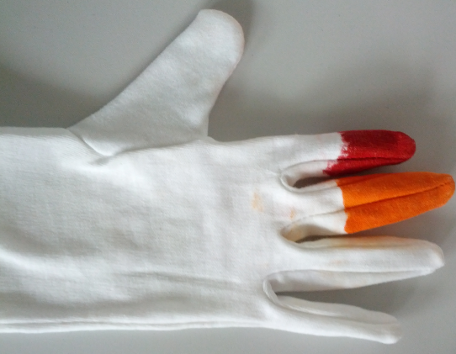
\includegraphics[width=7cm]{handschuh.png}

\begin{itemize}
	\item 100\% Baumwolle
	\item Hoher Tragekomfort
	\item Farbe: Orange
\end{itemize}
\end{frame}

\section{Algorithmen}

\subsection{Median Filter}
\begin{frame}
\frametitle{Median Filter}
\begin{itemize}
	\item Arbeitet auf dem Tiefenbild
	\item Filtert das Rauschen aus dem Tiefenbild heraus
\end{itemize}
\vspace*{1cm}
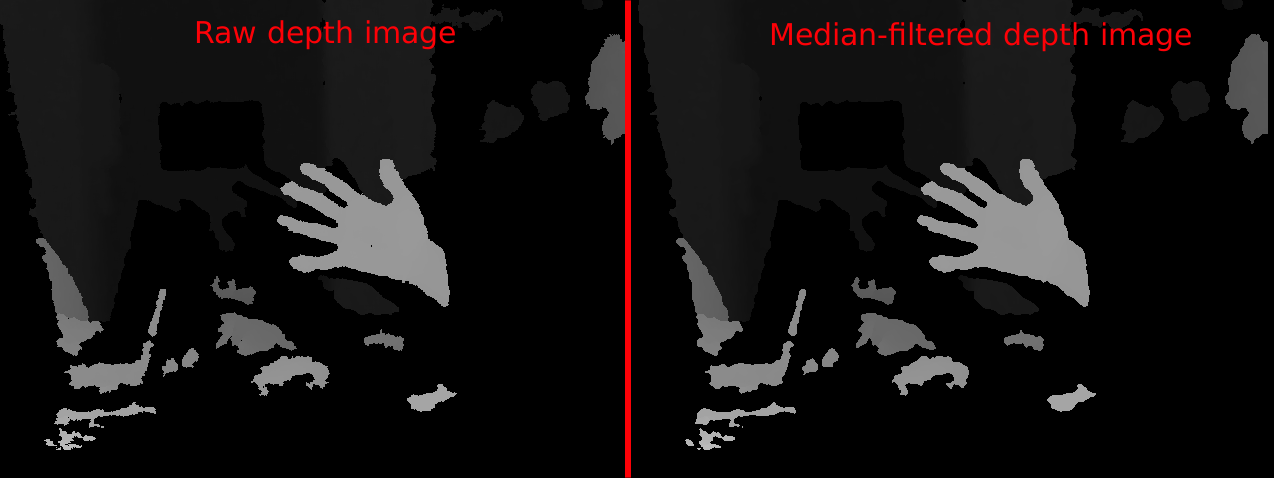
\includegraphics[width=12.4cm]{filter1.png}
\end{frame}

\subsection{Kalibrierung}
\begin{frame}
\frametitle{Kalibrierung}
\begin{itemize}
	\item Es kann auf neuen Hintergrund kalibriert werden
	\item Arbeitet auf dem Tiefenbild
	\item Filtert alle sich nicht bewegenden Punkte aus dem Tiefenbild.
\end{itemize}
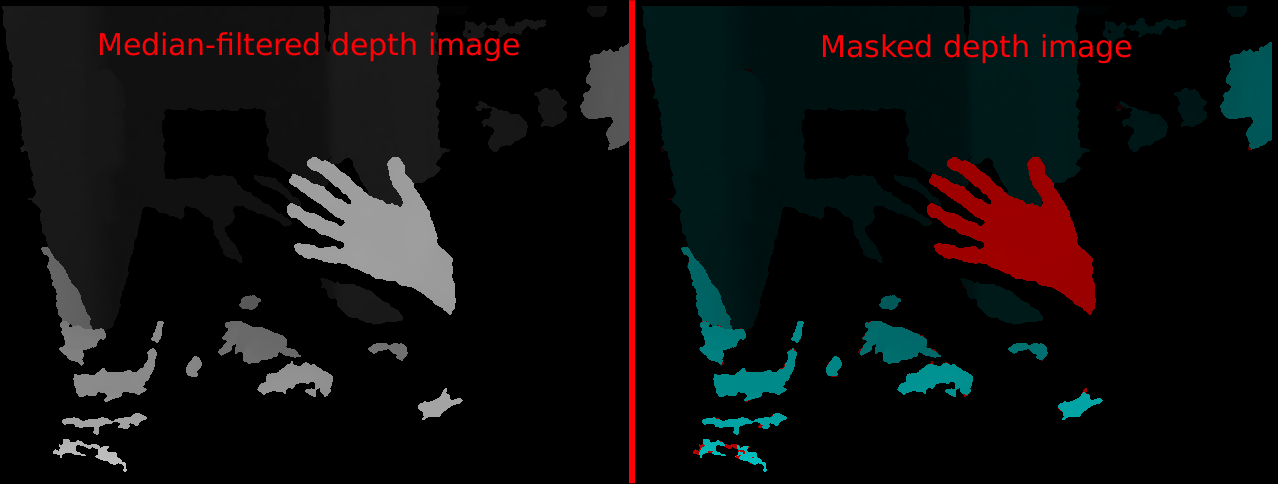
\includegraphics[width=12.4cm]{filter2.png}
\end{frame}

\subsection{Gloweffekt}
\begin{frame}
\frametitle{Gloweffekt}
\begin{itemize}
	\item Arbeitet auf dem Tiefenbild
	\item Expandiert alle anzuzeigenden Punkte im Tiefenbild, anhand eines einstellbaren Radius
\end{itemize}
\vspace*{0.5cm}
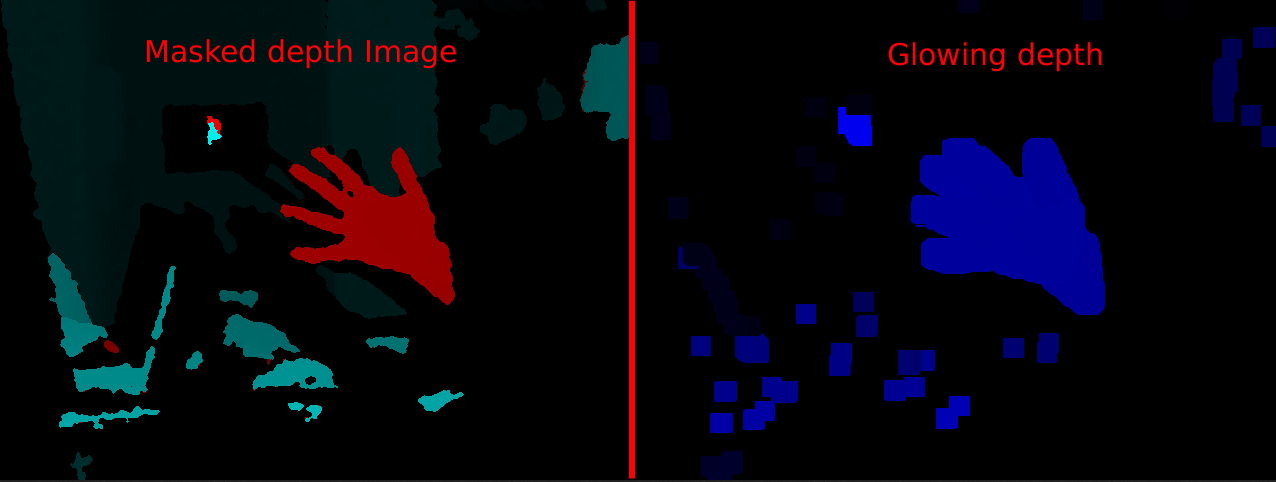
\includegraphics[width=12.4cm]{filter3.png}
\end{frame}

\subsection{RGB-Bild maskieren}
\begin{frame}
\frametitle{RGB-Bild maskieren}
\begin{itemize}
	\item Arbeitet auf dem RGB-Bild
	\item Rechnet das Tiefenbild auf das RGB-Bild um, und maskiert alle relevanten Pixel
\end{itemize}

\hspace*{2.2cm}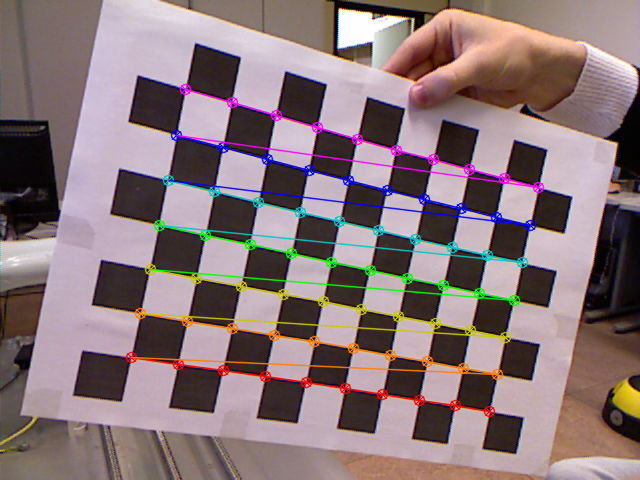
\includegraphics[width=7.5cm]{trans.png}
\end{frame}

\subsection{Referenz-Farbe}
\begin{frame}
\frametitle{Referenz-Farbe}
\begin{itemize}
	\item Arbeitet auf dem RGB-Bild
	\item Zeigt nur noch die Pixel auf dem RGB-Bild an, welche farblich ähnlich genug zur Referenzfarbe sind
\end{itemize}

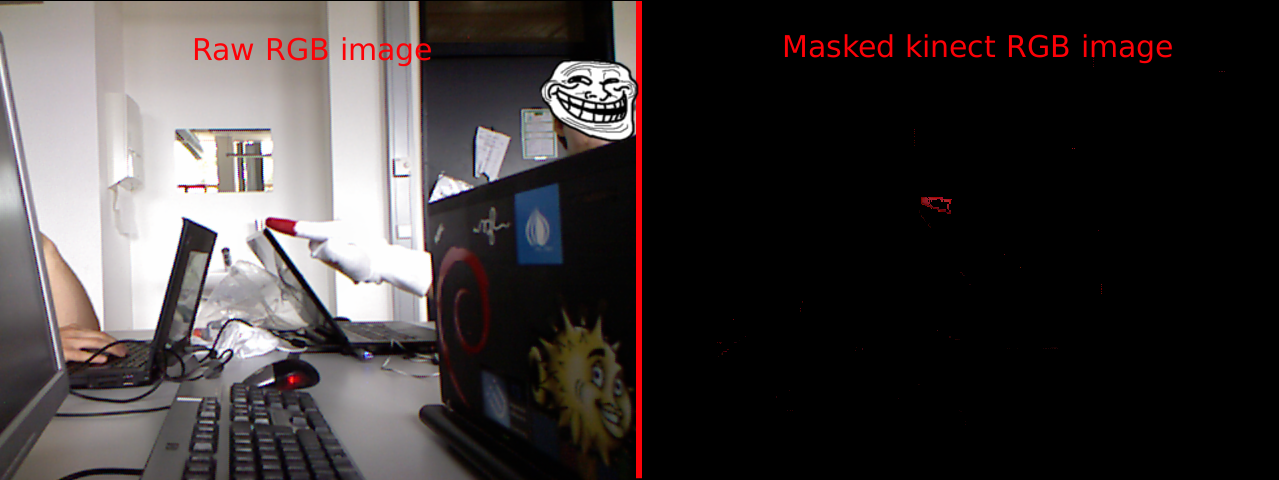
\includegraphics[width=12.4cm]{filter4.png}
\end{frame}

\subsection{Speed-Up}
\begin{frame}
\frametitle{Speed-Up}

{\Large $S(p)=\frac{\text{Ausführungszeit\, SingleCore}}{\text{Ausführungszeit\, MultiCore}}$}
\vspace*{0.4cm}
\setbeamercolor{block title}{bg=black,fg=orange}%bg=background, fg= foreground
\setbeamercolor{block body}{bg=boxgray,fg=black}%bg=background, fg= foreground
\begin{block}{Rechenzeit Tabelle}
	\begin{table}
		\begin{tabular}{|l|l|l|}
		\hline
		\textbf{Recheneinheit} & \textbf{Median Filter} & \textbf{RGB-Bild maskieren}\\
		\hline
		CPU & 30 Millisekunden & ? Millisekunden \\ \hline
		GPU & 1,5 Milisekunden & ? Mikrosekunden \\ \hline
		\end{tabular}
	\end{table}
\end{block}
\vspace*{0.4cm}
{\large
\begin{itemize}
	\item[] Speed-Up Median Filter: 5\%
	\item[] Speed-Up RGB-Bild-Maskierung: over9000\%
\end{itemize}
}

\end{frame}

\section{Portierung auf GPU}

\begin{frame}
\frametitle{Portierung auf GPU}
\begin{itemize}
\item Ausgangssituation (CPU)
	\begin{itemize}
		\item SDL Surface
		\item Softwarerendering
		\item 3 FPS bei einschalten der Filter
	\end{itemize}
\item Ziel (GPU)
	\begin{itemize}
		\item Bilder von Host auf Grafikkarte kopieren
		\item Bilder auf Grafikkarte berechnen
		\item Bilder von Grafikkarte auf Host kopieren
		\item extrem langsam 
	\end{itemize}
\end{itemize}
\end{frame}

\begin{frame}
\frametitle{Optimierung 1}
\begin{itemize}
\item Alle Bilder in einen Block
\item Weniger Memcopys
\item Immernoch zu langsam (5fps)
\item Kosten für ein Memcopy 7ms
\item Maximale Durchlaufdauer 30ms
\end{itemize}
\end{frame}

\begin{frame}
\frametitle{Optimierung 2}
\begin{itemize}
\item Hardwarerendering mit OpenGL
\item Spezielle OpenGL-Bufferobjekte
\item Nur noch kopieren der Input-Bilder erforderlich
\end{itemize}
\end{frame}

\begin{frame}
\frametitle{Optimierung 3}
\begin{itemize}
\item Doublebuffering verhindert flackern
\item BufferObjekt besteht aus front \& back
\item Bufferwechsel bei Pixelveränderung
\item VSync
\end{itemize}
\hspace*{4cm}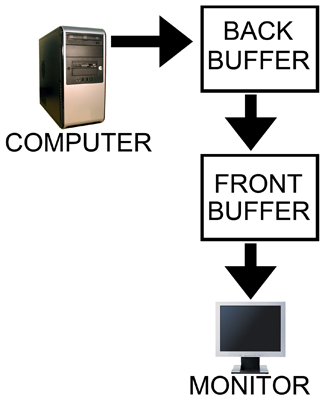
\includegraphics[width=3cm]{double.png}
\end{frame}

\begin{frame}
\frametitle{GPU GUI}
\begin{itemize}
\item Alte SDL-GUI keine OpenGL unterstützung
\item Awesomium
\end{itemize}
\hspace*{1,2cm}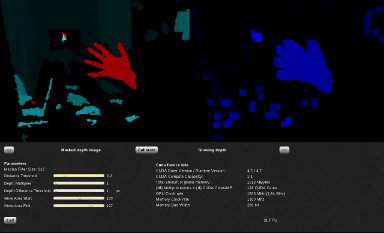
\includegraphics[width=10cm]{gui.png}
\end{frame}

\section{Ausblick}

\begin{frame}
\frametitle{Ausblick}
\begin{itemize}
	\item Bewegung interpolieren
	\item Extremitäten statt Pixel
	\item Visuell bedienbare GUI
	\begin{itemize}
		\item Buttons
		\item Gesten
	\end{itemize}
	\item Ausführlichere Dokumentation
	\item Plattformabhänigkeit minimieren
\end{itemize}
\end{frame}

\begin{frame}
\Huge
\centerline{Vielen Dank}
\centerline{für Ihre Aufmerksamkeit}
\end{frame}



\end{document}
